\section{Volume exploration space}
\label{sect:volume-exploration-space}
Figure~\ref{fig:tf-design-example} illustrates the TF design interface. This system interface is a 2D scatter plot. Each circle represents a pivot selected by SSS. The positions provided in the FastMap results determine the points' position in the scatter plot. A pivot represents a central point within a cluster. It assigns size as a pivot's secondary property. The radius of a circle is calculated based on the number of voxels it represents, normalized using a logarithmic scale.

\begin{figure*}[htb!]
    \centering
    \subfloat[Initial transfer function specification (semi-automatic generated).\label{subfig:tf-design-example-generated}]{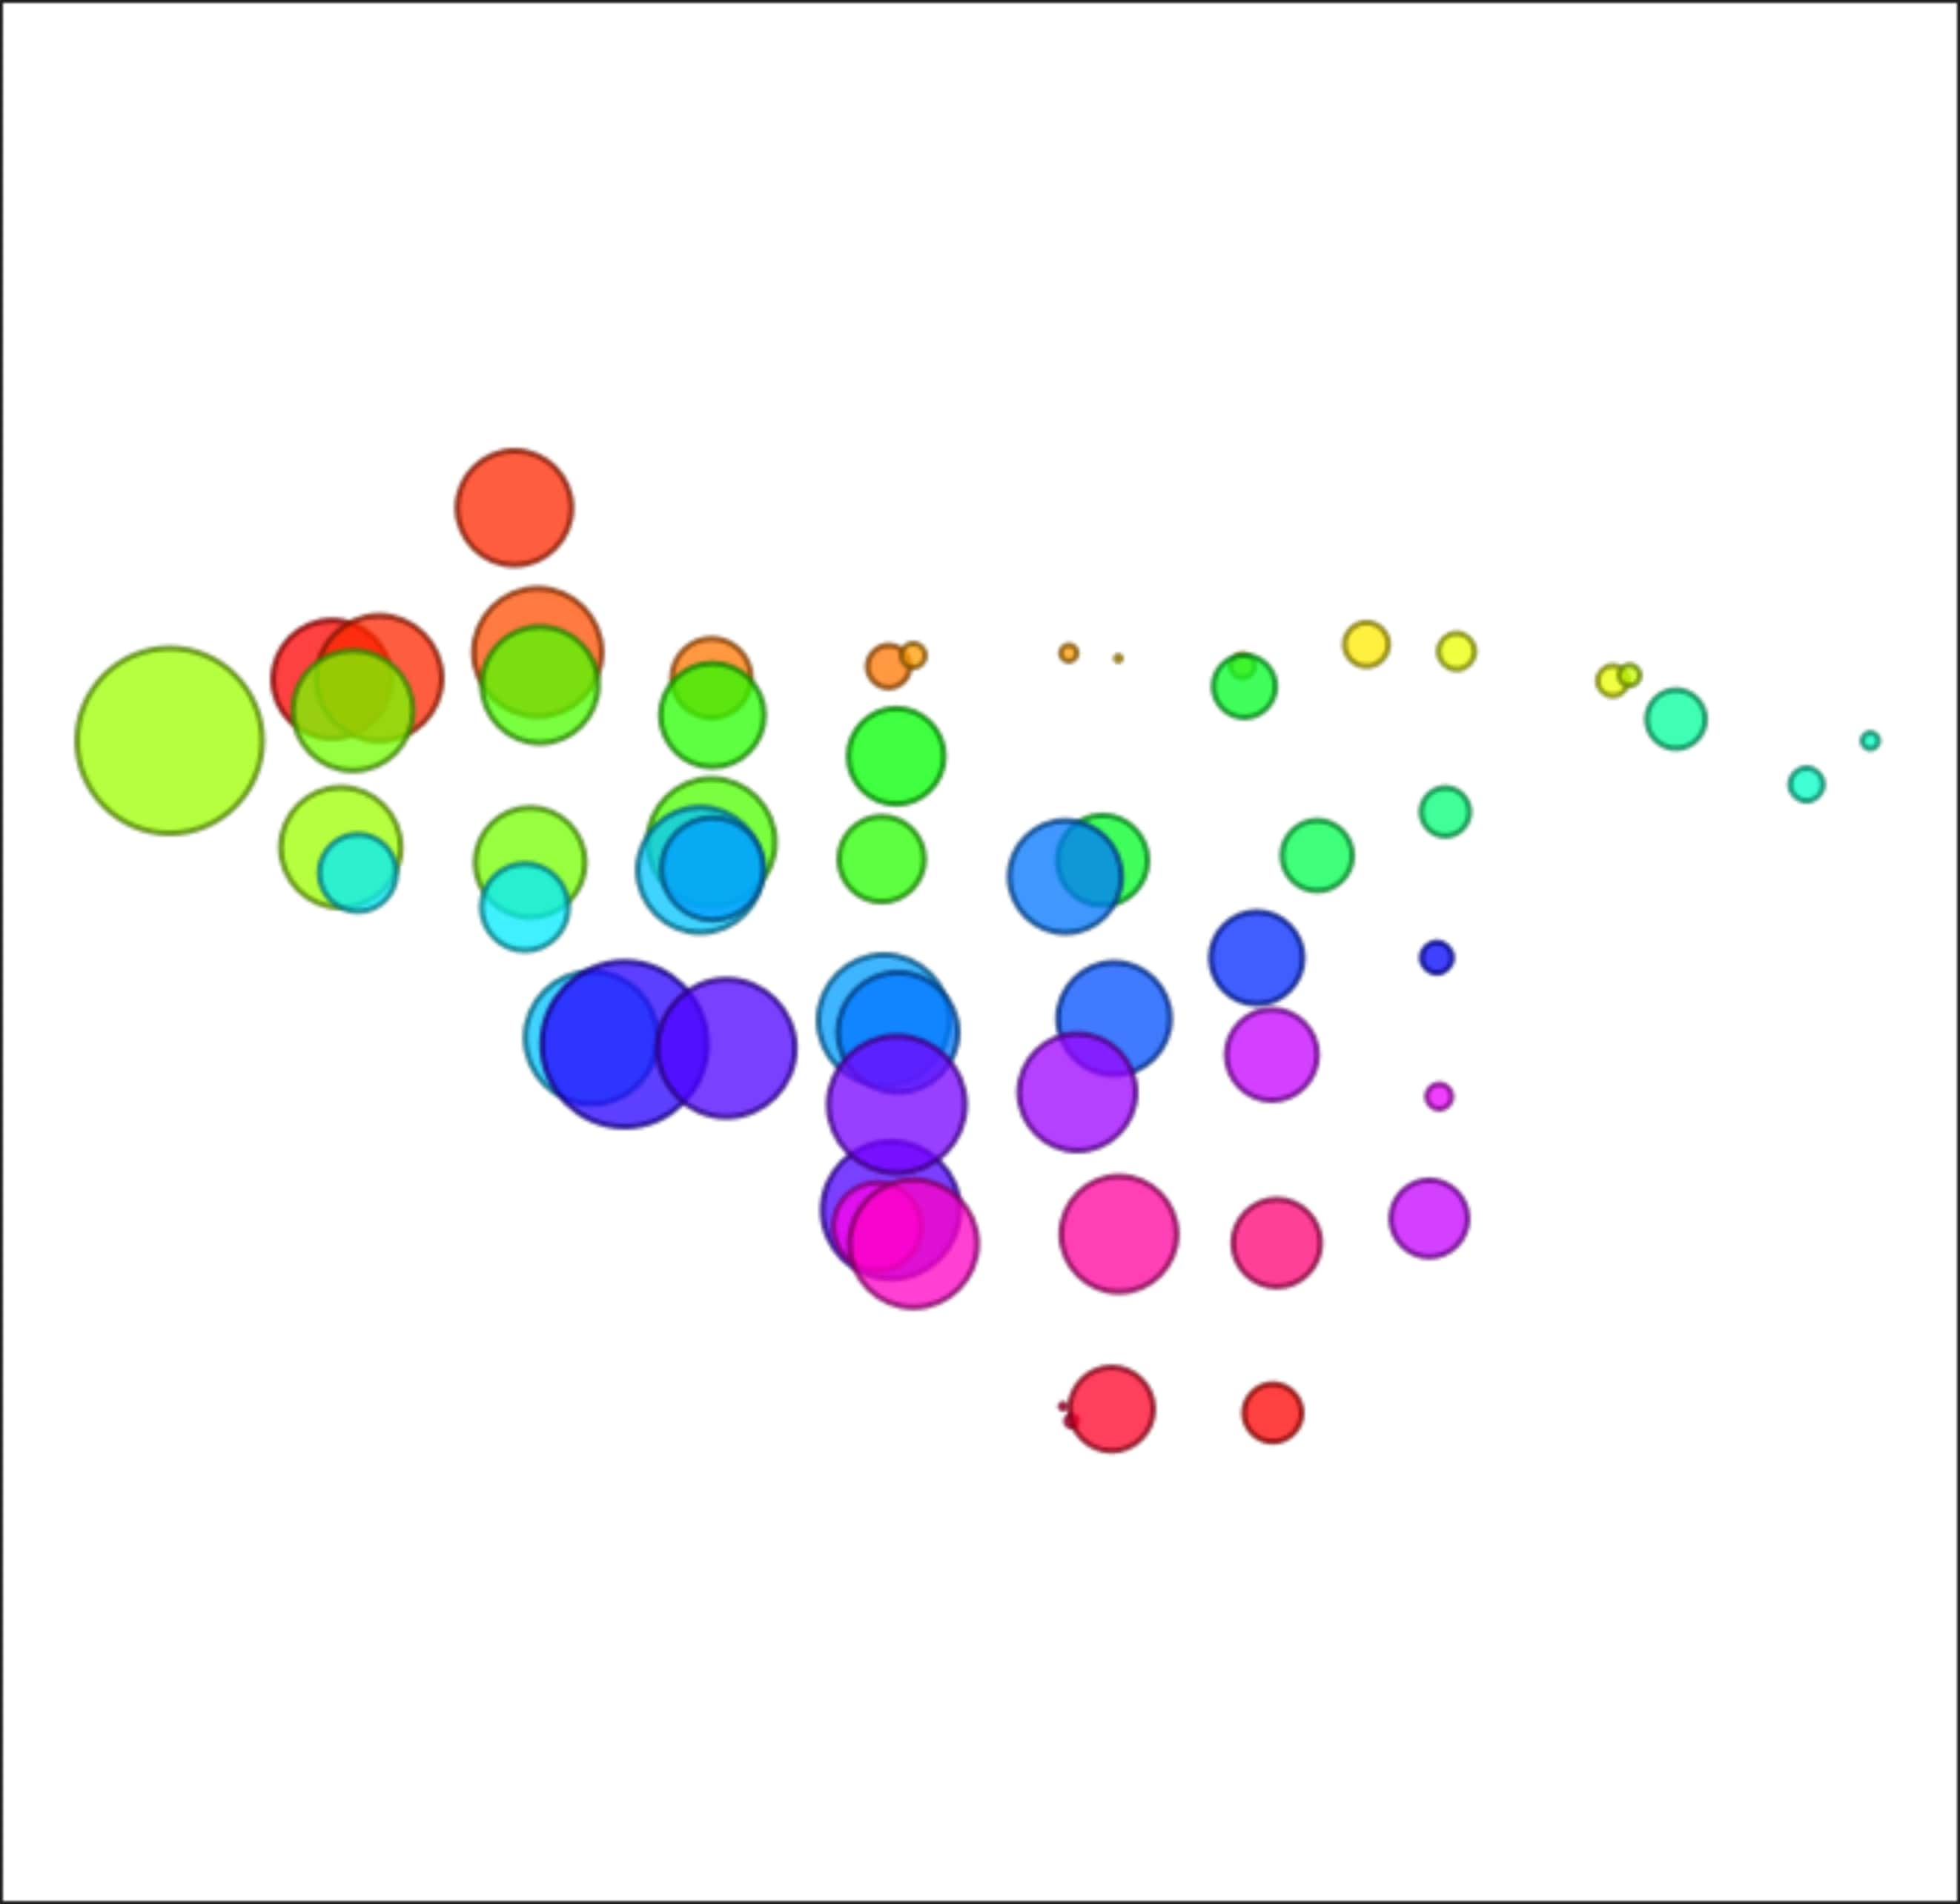
\includegraphics[width=0.9\columnwidth]{figs/tf-design-interface-a.jpg}}
    \hfill
    \subfloat[Fine-tune material classification after user adjustment.\label{subfig:tf-design-example-user}]{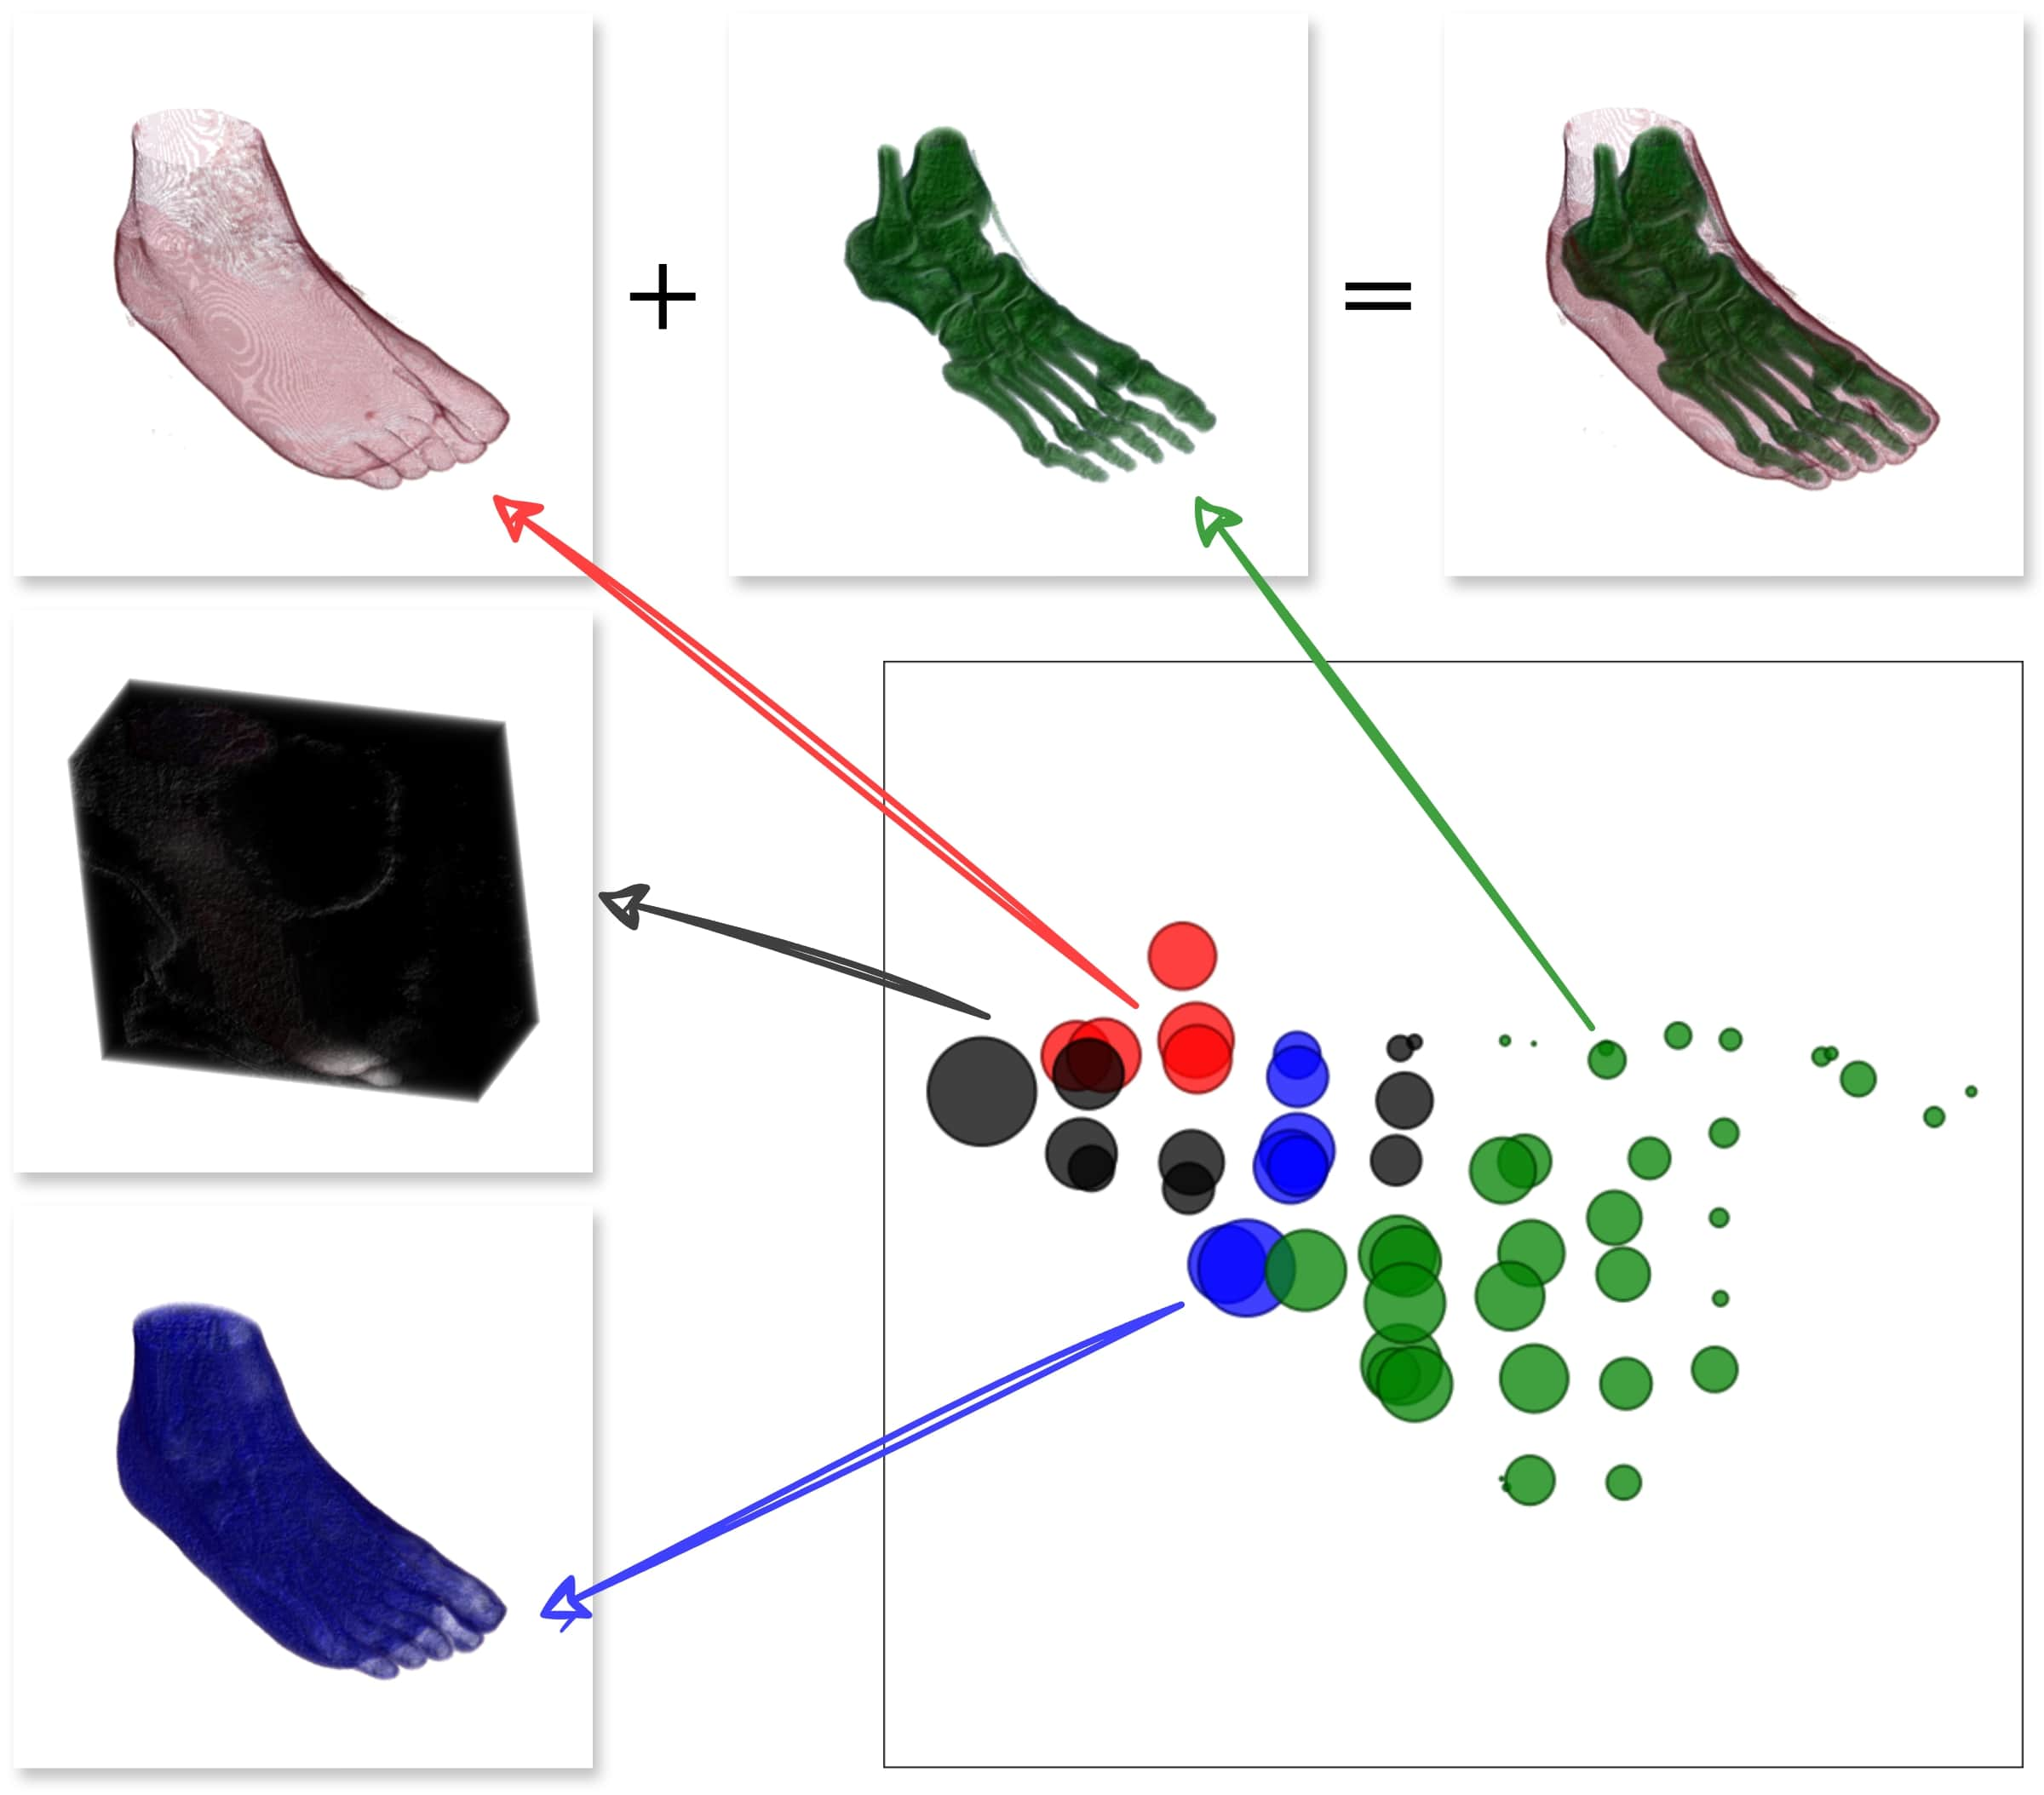
\includegraphics[width=0.9\columnwidth]{figs/tf-design-interface-b.jpg}}
\caption{Transfer function design interface and volume exploration space of a right male foot dataset.}
    \label{fig:tf-design-example}
\end{figure*}



Our approach generates an initial specification for the TF using a predefined opacity value alongside a rainbow color scale. Each cluster is assigned a unique color. 

Users can adjust the TF by following the What You See Is What You Get (WYSIWYG) principle. The lookup table is designed in such a way that the color and opacity of each pivot are directly mapped to the associated voxels, taking into account the clustering structure. Users can customize the color and opacity of any selected or not-selected elements.

Volume exploration happens through the selection of pivots. Our system dynamically adjusts the opacity of selected pivots to enhance visibility while concurrently reducing the opacity of non-selected elements. Users can interact with the system by making arbitrary selections. Even though hierarchical exploration is not the primary focus, our system supports it by enabling selections to be saved as groups, which can also be treated as selectable entities. This functionality empowers users to select pivots, clusters, and groups. 

The iterative selection of nearby elements is essential for identifying details and regions of interest inside a volume. FastMap and DBSCAN naturally group instances that are more similar closer together, simplifying the identification process.

Our approach automates material classification. Therefore, we assume that each cluster, or in a more sophisticated analysis, each pivot, represents a relevant item. If the user is unsatisfied with the result, they can go back to selecting or deselecting any element or adjust the method parameters, which are:

\begin{itemize}
    \item multidimensional TF definition,
    \item DBSCAN $\varepsilon$ and $minPts$, and
    \item SSS distance factor $\alpha$.
\end{itemize}